\section{Introduction}\label{sec:page-layout}
The rapid advancement of reinforcement learning (RL), especially through the development and application of Deep Q-Networks (DQN). DQN is a prominent RL algorithm that utilizes deep learning techniques to approximate Q-values, which are critical for predicting the expected future rewards of taking specific actions in given states. This capability is essential for training agents to perform tasks that involve sequential decision-making and dynamic environments.

This paper presents an approach to train an agent to play the Atari Video Pinball game using the Double DQN algorithm. Atari games are renowned for their complexity and serve as a challenging benchmark for assessing the performance and robustness of RL algorithms. The methodology employed includes the preprocessing of game frames to provide the agent with meaningful input data, the implementation of an epsilon-greedy strategy to balance exploration and exploitation during action selection, and the utilization of a replay memory to store and sample experiences for effective training.

The experimental results demonstrate the agent’s capacity to learn effective policies through iterative interactions with the game environment. A detailed analysis of the training process, the challenges encountered, and potential improvements to enhance the agent’s performance is provided. 
\begin{comment}
The rapid advancement of artificial intelligence (AI) and machine learning (ML) has significantly propelled the field of reinforcement learning (RL), especially through the development and application of Deep Q-Networks (DQN). DQN is a prominent RL algorithm that utilises deep learning techniques to approximate Q-values, which are critical for predicting the expected future rewards of taking specific actions in given states. This capability is essential for training agents to perform tasks that involve sequential decision-making and dynamic environments.

\begin{figure}[!h]
\centering
\centerline{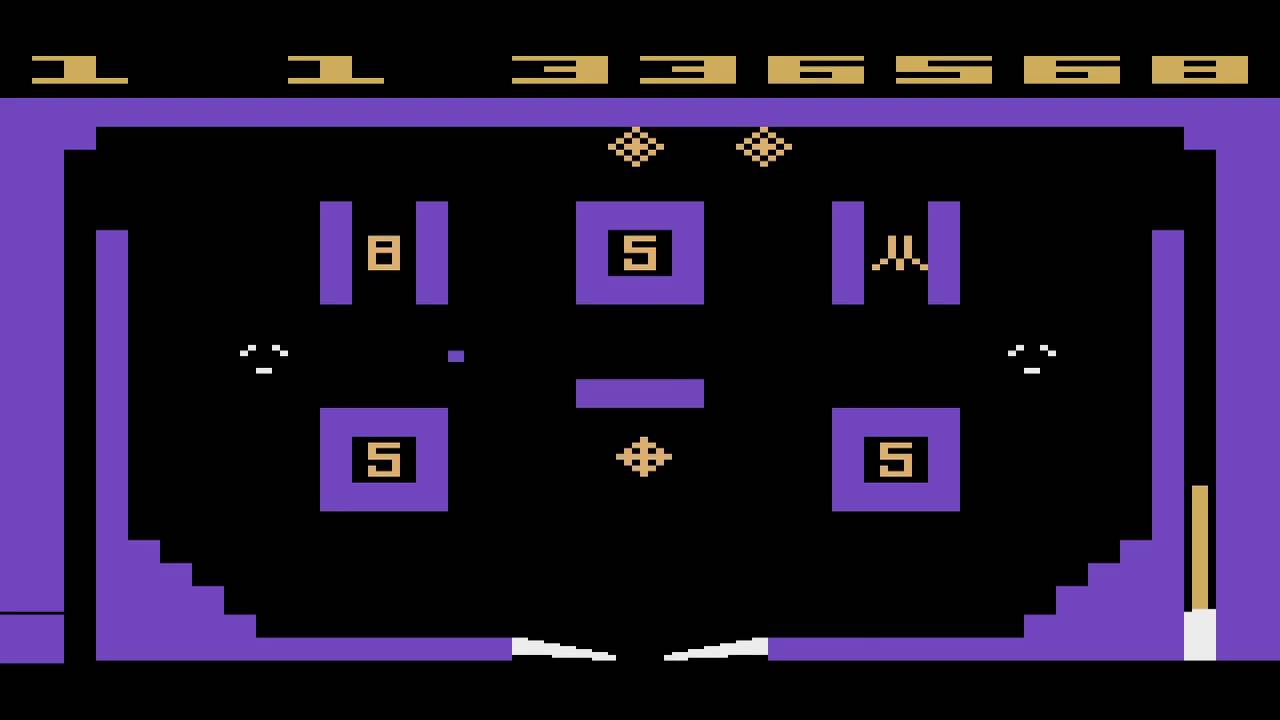
\includegraphics[scale=0.17]{graphics/game.jpg}}
\caption{This figure presents a demo of the actual game.}
\label{fig: game}
\end{figure} 

This paper presents an approach to train an agent to play the Atari Video Pinball game using the DQN algorithm. Atari games are renowned for their complexity and serve as a challenging benchmark for assessing the performance and robustness of RL algorithms. The methodology employed includes the preprocessing of game frames to provide the agent with meaningful input data, the implementation of an epsilon-greedy strategy to balance exploration and exploitation during action selection, and the utilisation of a replay memory to store and sample experiences for effective training.

The experimental results demonstrate the agent’s capacity to learn effective policies through iterative interactions with the game environment. A detailed analysis of the training process, the challenges encountered, and potential improvements to enhance the agent’s performance is provided. This study contributes to the field of reinforcement learning by offering insights into the practical application of DQN in complex environments such as Atari games. It thus advances our understanding of the algorithm’s strengths and limitations in real-world scenarios.
\end{comment}

